% §5 Experiments. Every number is traceable to a file under results/ (comment next to the claim).
% The longer pre-condensation draft is kept in sections/experiments_long.tex.bak.
\section{Experiments}
\label{sec:experiments}

We test four things: that each width responds to the acquisition it is built to track
(\cref{sec:exp-synthetic}), that the joint intervals include their targets on frozen real features
(\cref{sec:exp-real}), whether the widths choose an acquisition that pays under shift
(\cref{sec:exp-blindspot}), whether the exchange rate of \cref{sec:theory} chooses the better
acquisition when the class-conditionals hold (\cref{sec:exp-exchange}), and whether a per-input
attribution names the source that actually limits the certified interval (\cref{sec:exp-attribution}).
Each test's expected outcomes were registered in the code before it ran; every registered outcome,
including the failures, is in \cref{app:outcomes}, and deviations are listed in \cref{app:deviations}.

\subsection{Protocol}
\label{sec:exp-protocol}

\paragraph{Response slopes.} For each acquisition we sweep its budget on a log-spaced grid with the
other two at base values, and fit the least-squares slope of $\log(\text{mean width})$ on
$\log(\text{budget})$, so $-1/2$ is the parametric rate. Confidence intervals bootstrap over seeds,
the independent replicate. A slope is called ``$\approx0$'' when it lies inside the
$1-\alpha/K$ quantile ($\alpha=0.05$, Bonferroni over the $K$ registered cells) of slopes refitted
on fresh same-budget seeds randomly assigned to grid levels. This is a failure to reject against a
placebo null for that estimator at that seed count, not an equivalence test: it says the response is
not distinguishable from Monte Carlo noise; the tolerance $\tau$ of every cell is in the released
response matrices so its power is visible. Results are conditional on one fitted head and one test pool
per encoder, and we make no multiplicity correction across sections.
Invariances that hold by construction are marked $0^{\ast}$. Before any slope is reported the pipeline checks that the ball resolves a $0.4$
shift of weight between the two closest sources, $\lVert0.4(\hat A_i-\hat A_j)\rVert/(\varepsilon_n+r)>1$,
at the smallest $n$.

\paragraph{Baselines.} EMQ \citep{saerens2002adjusting} with a multinomial bootstrap of the log gives
percentile intervals for the same estimands as $\Wcls$ and $\Wunk$, without a finite-sample guarantee.
A bootstrap ensemble that resamples both the log and the labels gives ensemble mutual information
$\mathrm H(\bar p)-\overline{\mathrm H(p)}$, the scalar score the introduction argues against.

\subsection{Synthetic response matrix}
\label{sec:exp-synthetic}

Three sources over four cells: two known sources and a novel one with mass $\delta=0.1$, label rates
$\theta=(0.2,0.8,0.9)$. Probe cells are \emph{on support}, \emph{boundary} (known-source overlap) and
\emph{off support} (zero mass). The novel source lies outside the known hull in world
\emph{separated}, at the midpoint of the known rows in \emph{confounded}, and is absent in
\emph{absent}. Grids are $n\in\{2^{10},\dots,2^{16}\}$, $m\in\{2^5,\dots,2^{11}\}$,
$\eta\in\{0.0125,\dots,0.2\}$, 128 seeds per budget; the resolution gate reads $2.44$.

\begin{table}[t]
\centering\small
\caption{Response matrix, world \emph{separated}, on-support probe: log-log slope of mean width
against each acquisition. Arrows: outside the placebo band; $0^{\ast}$: invariant by construction; the $\Wlab$ arrows follow from its
closed-form radius.
Bootstrap half-widths $<0.03$.}
\label{tab:synthetic}
\resizebox{\columnwidth}{!}{% generated from results/response_l2_s128/response_matrix.csv (world=separated, region=on_support)
\begin{tabular}{lccc}
\toprule
 & unlabelled log $n$ & labels $m$ & noise $\eta$ \\
\midrule
\Wcls & $-0.51$ $\downarrow$ & $0^{\ast}$ & $0^{\ast}$ \\
\Wlab & $0^{\ast}$ & $-0.47$ $\downarrow$ & $+0.16$ $\uparrow$ \\
\Wunk & $-0.49$ $\downarrow$ & $0^{\ast}$ & $0^{\ast}$ \\
\midrule
EMQ+bootstrap & $-0.50$ $\downarrow$ & $0^{\ast}$ & $0^{\ast}$ \\
Ensemble MI & $-0.03$ $\downarrow$ & $-0.82$ $\downarrow$ & $+0.44$ $\uparrow$ \\
\bottomrule
\end{tabular}
}
\end{table}

\Cref{tab:synthetic} shows the predicted pattern. $\Wcls$ contracts with the log at the parametric
rate (slope $-0.51$, 95\% CI $[-0.508,-0.503]$), $\Wlab$ contracts with labels ($-0.47$) and widens
with noise ($+0.16$), and $\Wunk$ contracts with the log ($-0.49$) on support and stays at $1$ off
support. Ensemble MI responds to all three ($-0.03$, $-0.82$, $+0.44$) and barely registers the log, although the
prevalence width falls eightfold over the same grid. Of the 25 registered cells, 12 concern the baselines (all agree) and 13 concern REACH. Of
those, two are off-support cells that are $[0,1]$ by policy and four follow from the closed-form
label radius, so neither group is evidence; of the remaining seven, five agree (prevalence and
coverage contraction) and two do not. Both failures are the coverage width in \emph{confounded},
registered as no response: the width stays large ($1.0\to0.69$ on support,
$0.86$ on the boundary at $n=2^{16}$) but falls with slope $-0.09$ and $-0.04$, as the ball shrinks
onto a wide identified set. ``Attenuated fivefold, bounded below'', as \cref{prop:c}(ii) states,
would have been the right registration; a later registered dose-response study with $K=4$ fixed confirms
that form ($\Wunk$ falls with $s$, Spearman $-0.97$, and at $s=0$ its log-slope in $n$ is only $-0.10$, leaving
it at $0.43$ for $n=1.28\times10^5$; \cref{app:outcomes}). Prevalence also contracts more slowly there ($-0.35$ on support), as $\sigma=0$ predicts. The ball contains the true marginal in every
seed at every $n$ (Clopper--Pearson lower bound $0.977$ at nominal $0.975$). EMQ+bootstrap is about
three times narrower and near nominal in \emph{separated} ($0.92$--$0.96$), but in
\emph{confounded} its coverage falls from $0.73$ to $0$: EM picks one point of a non-identified set
and the bootstrap shrinks around it (\cref{fig:coverage}, left).
% results/response_l2_s128/{response_matrix.csv,summary.json}

\subsection{CIFAR-10 audit with frozen encoders}
\label{sec:exp-real}

CIFAR-10 images \citep{krizhevsky2009learning} pass through a frozen CLIP ViT-B/32
\citep{radford2021clip}; PCA to 32 dimensions and an
equal-prior Gaussian LDA head are fitted on $10{,}000$ training images (accuracy $91.2\%$). Rows are
estimated from $m$ of the remaining $40{,}000$ per source, and the log is drawn from the test set. With
one source per class the ball cannot resolve classes whose deployment mass is below its radius (about
$0.10$ at $m=2000$), so the headline uses four superclass sources with fixed within-group composition
(which makes frozen class-conditionals hold by construction for label shift); ten sources are reported
alongside. Both pass the resolution gate ($1.14$, $1.62$). Label-shift and held-out arms use 50 seeds
and Dirichlet(1) prevalences drawn per seed; coverage is judged at the solver's accuracy ($10^{-6}$).
Two interval baselines join EMQ: a constraint region after \citet{li2026matrix}, built from per-cell
intervals on the log frequencies and the same per-entry intervals on the rows, with no ball; and a
two-stage bootstrap that resamples the references as well as the log.

\begin{table}[t]
\centering\small
\caption{CIFAR-10 label shift, CLIP, $n=16{,}000$, $m=2000$, 50 seeds: per-probe inclusion of the true
posterior (column ``coverage'') and mean width on known-class cells.}
\label{tab:real}
\setlength{\tabcolsep}{4pt}
\resizebox{\columnwidth}{!}{% generated from results/audit_v3_clip_{super4,classes}_lsho/summary.json (label_shift, on_support, n=16000)
\begin{tabular}{lcccc}
\toprule
 & \multicolumn{2}{c}{4 superclass sources} & \multicolumn{2}{c}{10 class sources} \\
\cmidrule(lr){2-3}\cmidrule(lr){4-5}
 & coverage & width & coverage & width \\
\midrule
REACH joint interval & 1.00 & 0.71 & 1.00 & 0.88 \\
Constraint region (after Li et al.) & 1.00 & 0.65 & 1.00 & 0.74 \\
EMQ, two-stage bootstrap & 0.82 & 0.06 & 0.58 & 0.07 \\
EMQ, log-only bootstrap & 0.13 & 0.01 & 0.17 & 0.03 \\
REACH $\Wcls$ (plug-in) & 0.98 & 0.46 & 1.00 & 0.76 \\
\bottomrule
\end{tabular}
}
\end{table}

\paragraph{Coverage and width.} Both finite-sample constructions include the target in every seed at every
$n$, for both groupings (\cref{tab:real}), and at $n=16{,}000$ the constraint region is narrower than or
equal to REACH's joint interval on every probe (on average $0.65$ against $0.71$ with super4 sources, $0.74$
against $0.88$ with ten). Neither is informative in absolute terms: $41\%$ of super4 joint intervals are
$[0,1]$ ($68\%$ with ten sources). The tight joint interval of \cref{sec:setup} closes $56$--$71\%$ of the gap
to the region. Log-only EMQ covers $0.54$ at $n=500$ and $0.13$ at $n=16{,}000$, because reference error is
ignored (\cref{fig:coverage}, centre); resampling the references as well lifts it to $0.82$. Plug-in $\Wcls$
includes the target in $0.98$ of probes ($0.94$ with DINOv2) without a guarantee, which is why the joint
interval carries the claim.
% results/audit_v3_clip_{super4,classes}_lsho/summary.json n_axis_coverage

\paragraph{Response.} All 13 registered cells agree for super4 (12 of 13 with ten sources). But on real
data the joint width responds to all three acquisitions ($-0.07$ in $n$, $-0.11$ in $m$, $+0.04$ in $\eta$),
and labels also narrow $\Wcls$ ($-0.19$), because labels estimate the rows the ball is built from; one-to-one
attribution by width does not hold, which \cref{sec:exp-exchange,sec:exp-attribution} take up. Ensemble MI
responds to the log and to labels but not to label noise.
% results/audit_v3_clip_super4_lsho/response_matrix.csv

\paragraph{Unseen classes and corruption.} With ship and truck withheld from the labelled set ($s=0.22$)
and present as $\delta=0.1$ of the log, or absent, the joint coverage interval includes its target in every
seed and contracts in both arms ($0.92\to0.72$, $0.89\to0.66$); plug-in $\Wunk$ under-covers with DINOv2
($0.88$). A declared uniform unseen component is never flagged, so we make no claim that the audit detects a
wrong unseen model. On CIFAR-10-C \citep{hendrycks2019benchmarking} the rows move; REACH abstains when the
ball is empty, answering $94\%$ of super4 runs at severity 1 and $45\%$ at severity 5, and includes the
target in $0.998$ and $0.93$ of those it answers; the constraint region answers $26\%$, and bootstrap EMQ
includes $0.21$. Ten super4 corruption-severity cells under-cover, mostly with the test silent; DINOv2
\citep{oquab2024dinov2} reproduces every pattern (\cref{app:extra}).
% results/audit_v3_clip_{super4,classes}_corruption/summary.json severity, severity_by_corruption

\begin{figure*}[t]
\centering
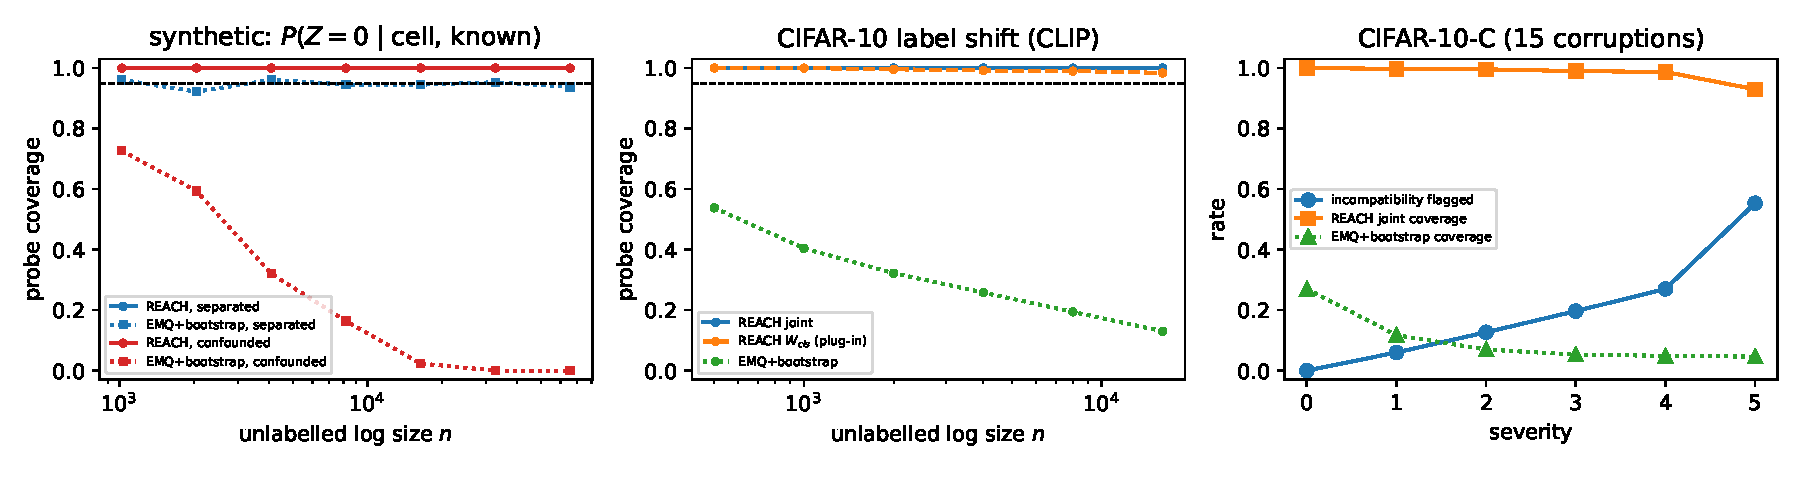
\includegraphics[width=\textwidth]{figures/fig3_coverage.pdf}
\caption{Per-probe inclusion of REACH and EMQ+bootstrap. Left: synthetic; both REACH curves lie on
$1.0$. Centre: CIFAR-10 label shift, four superclass sources. Right: CIFAR-10-C pooled over 15
corruptions, inclusion among runs where the ball is not empty, with the rate at which the
incompatibility test fires. Constraint-region and two-stage-bootstrap results are in the text.
Dashed: $0.95$.}
\label{fig:coverage}
\end{figure*}

\subsection{Does the width comparison choose the data that pays?}
\label{sec:exp-blindspot}

Without ground-truth widths this test is behavioural: take the acquisition REACH recommends per cell
and measure what it buys on held-out shifted data. Shift splits are clean CIFAR-10, CIFAR-10.1
\citep{recht2018cifar} and the 75 CIFAR-10-C splits, each cut into disjoint log, label and evaluation
pools. An episode draws Dirichlet(1) prevalences over the superclasses and starts from clean rows
($m=2000$) and $1000$ shifted log images. With budget $5000$ units, \emph{reweight} grows the log to
$6000$ and refits EMQ; \emph{add labels} buys $5000/c$ shifted labels and shrinks the rows towards them
($M_0=50$); \emph{do nothing} has payoff $0$. Payoff is the reduction of held-out negative
log-likelihood (nats) in a cell; regret is the best action's payoff minus the chosen one's. We compare
REACH (\cref{sec:setup}) with every constant policy, the incompatibility flag alone, and ensemble MI
mapped to actions by tercile with the map tuned on calibration-seed regret. Seeds 10--19 are
evaluated; intervals use a two-way cluster bootstrap over seeds and shift families. This is the second registered version of the test; the first had rule defects that review exposed
(\cref{app:deviations}).

\begin{table}[t]
\centering\small
\caption{Mean regret (nats per cell) by policy. Left: price 1:50 by shift family; right: all 77
splits at prices 1:50 and 1:250. Evaluation seeds; prior strength $M_0=50$.}
\label{tab:blindspot}
\setlength{\tabcolsep}{3pt}
\resizebox{\columnwidth}{!}{% generated from results/blindspot_v2/summary.json (evaluation seeds 10-19; prereg sha 2fdecf48)
\begin{tabular}{lrrrrr}
\toprule
 & \multicolumn{3}{c}{price 1:50, by family} & \multicolumn{2}{c}{all splits} \\
\cmidrule(lr){2-4}\cmidrule(lr){5-6}
policy & clean & C10.1 & C10-C & 1:50 & 1:250 \\
\midrule
REACH-v2 & 0.0029 & 0.0101 & 0.0864 & 0.0843 & 0.0411 \\
flag only & 0.0026 & 0.0096 & 0.0877 & 0.0856 & 0.0429 \\
always labels & 0.0086 & 0.0188 & 0.0100 & 0.0101 & 0.0084 \\
always reweight & 0.0019 & 0.0074 & 0.2382 & 0.2321 & 0.1189 \\
do nothing & 0.0018 & 0.0083 & 0.2401 & 0.2340 & 0.1208 \\
\bottomrule
\end{tabular}
}
\end{table}

\paragraph{Result.} The registered prediction fails: buying labels every time has lower regret than
REACH at every price ($0.010$ against $0.084$ at 1:50, difference CI $[0.038,0.134]$; $0.008$ against
$0.041$ at 1:250, $[0.014,0.063]$) and at every prior strength $M_0\in\{10,50,200\}$, and the regret-tuned
MI map is the same constant policy. The reason follows from the registered rule itself: under frozen
class-conditionals the predicted label gain can only widen the rows' radius when $n_k<m$ (true at every
price), so in a compatible frame REACH never predicts that labels help (largest predicted label gain $3\times10^{-8}$ at 1:50, $6\times10^{-8}$
over all settings). All of its label recommendations therefore come from the incompatibility test, which fires in only $33\%$ of
severity-5 episodes, while shifted labels pay $0.23$ nats under corruption. On clean CIFAR-10 and
CIFAR-10.1, where labels slightly hurt ($-0.007$ and $-0.011$ nats), REACH beats always-labels but not
doing nothing, always reweighting or the flag alone (\cref{tab:blindspot}); beyond the flag the width
comparison adds nothing (REACH minus flag-only within $[-0.005,0.0005]$ at 1:50). Under shift the widths
cannot tell whether the rows have moved.
% results/blindspot_v2/{summary.json,rows.csv.gz}; prereg real/blindspot_prereg_v2.py sha 2fdecf48

\subsection{When the class-conditionals hold: the exchange rate chooses the data}
\label{sec:exp-exchange}

Under frozen class-conditionals the question is which acquisition tightens a certified interval more at
a given price. Registered before its code and before a third encoder existed: $n_0\in\{500,2000,8000\}$,
$m_0\in\{125,500,2000\}$ ($\{32,128,512\}$ in a synthetic world with estimated rows), prices
$c\in\{10,50,250\}$, budget $5000$; the outcome is the realised reduction of the mean tight joint width.
REACH re-solves the tight interval at the post-acquisition radii; the data-free alternative compares the
radius reductions alone. Primary settings: the synthetic world and a frozen ResNet-50 \citep{he2016deep}
never inspected before the run; CLIP replicates; seeds 10--29 evaluated.

\begin{table}[t]
\centering\small
\caption{Exchange-rate test under pure label shift: which acquisition tightens the certified interval
more. Regret in width units, evaluation seeds; CI: seed bootstrap.}
\label{tab:exchange}
\setlength{\tabcolsep}{3pt}
\resizebox{\columnwidth}{!}{% generated from results/exchange_{synthetic,resnet50,clip}/summary.json and rows.csv.gz (prereg a70683e3)
\begin{tabular}{lccc}
\toprule
 & synthetic & ResNet-50 & CLIP \\
 & (blind) & (blind) & (seen) \\
\midrule
cells where labels are better & 14/27 & 4/27 & 4/27 \\
predicted sign correct & 1.00 & 1.00 & 1.00 \\
corr.\ predicted vs realised gain & 0.995 & 0.999 & 1.000 \\
\midrule
regret: REACH & 0.0019 & 0.0001 & 0.0001 \\
\quad radius bookkeeping & 0.0019 & 0.0000 & 0.0001 \\
\quad always log & 0.0540 & 0.0032 & 0.0035 \\
\quad always labels & 0.0487 & 0.0411 & 0.0426 \\
\quad ensemble MI (tuned) & 0.0224 & 0.0032 & 0.0035 \\
REACH $-$ best constant, 95\% CI & $[-0.0514,-0.0424]$ & $[-0.0036,-0.0026]$ & $[-0.0040,-0.0028]$ \\
\midrule
tight width (vs.\ region) & 0.83 (0.79) & 0.90 (0.89) & 0.89 (0.88) \\
tight $\le$ joint, share of probes & 1.00 & 1.00 & 1.00 \\
tight inclusion (min over bases) & 1.00 & 1.00 & 1.00 \\
\bottomrule
\end{tabular}
}
\end{table}

\paragraph{Result.} All registered claims hold (\cref{tab:exchange}), but what they establish is
narrower than the registration suggests. The better acquisition changes across base points and prices
in 14 of 27 synthetic cells and 4 of 27 real ones (labels win when the log is already large, references are
few and labels cheap), and REACH picks it, with regret below both constant policies and the tuned MI map
(CIs exclude zero in all three settings). Three qualifications. First, the decision value is the radius
exchange rate's: the data-free comparison of radii makes the same choice in $93$--$94\%$ of episodes with
regret equal to or lower than REACH's, and the choice is per deployment, not per input. Second, on real
features the stakes are small: ``always more log'' is right in 23 of 27 cells and trails by $0.003$ width
units on intervals about $0.9$ wide, and $29$--$32\%$ of episodes have mean width $\ge0.999$. Third, the
prediction re-solves the same program (partly a self-consistency check), and the tight interval, which
\cref{prop:bprime} does not cover, includes the target in every seed but stays wider than the constraint
region ($0.90$ against $0.89$ on ResNet-50).
% results/exchange_{synthetic,resnet50,clip}/summary.json; prereg real/exchange_prereg.py sha a70683e3

\subsection{Which source limits the certified interval?}
\label{sec:exp-attribution}

Attribution claims a per-input answer, so we score it against one. At each probe an \emph{oracle} removes
one source at a time from the tight joint interval (true marginal with tolerance $0$; true rows; true
$\delta$); the source whose removal narrows the interval most is the truth, scored where some removal narrows
it by at least $0.01$. Regret is the oracle's best narrowing minus that of the named source. The comparator
\emph{budget-majority} names the most frequent oracle source at the same setting and budget, learned with
hindsight on calibration seeds. Settings: the label-shift and held-out arms of \cref{sec:exp-real} with three
encoders (each CIFAR-10 class held out in turn; five CIFAR-100 superclasses), Gaussian features in
$\mathbb R^{64}$ through the same head, and classifier-like categorical worlds (\cref{app:details}).

\begin{table}[t]
\centering\small
\caption{Oracle regret (width units, evaluation seeds; on real data never run before the test was
registered) of naming the limiting source. Raw widths: argmax of $(\Wcls,\Wlab,\Wunk)$. Last data row: the realised
narrowing from acquiring $4\times$ more log or labels. CI: two-way bootstrap over seeds and settings.}
\label{tab:attribution}
\setlength{\tabcolsep}{3pt}
\resizebox{\columnwidth}{!}{\begin{tabular}{lcccc}
\toprule
 & raw widths & budget-majority & REACH-pin & pin $-$ majority [95\% CI] \\
\midrule
C10 held-out, 3 encoders & 0.284 & 0.045 & 0.0016 & $-0.043$ $[-0.047, -0.039]$ \\
C10 label shift, 3 encoders & 0.361 & 0.014 & 0.0012 & $-0.013$ $[-0.020, -0.007]$ \\
C100 held-out, CLIP & 0.400 & 0.009 & 0.0115 & $+0.002$ $[-0.003, +0.008]$ \\
C100 held-out, DINOv2 & 0.404 & 0.009 & 0.0028 & $-0.007$ $[-0.008, -0.005]$ \\
C100 label shift, CLIP & 0.307 & 0.001 & 0.0126 & $+0.011$ $[+0.005, +0.018]$ \\
C100 label shift, DINOv2 & 0.267 & 0.002 & 0.0041 & $+0.002$ $[-0.000, +0.005]$ \\
Gaussian features, held-out & 0.213 & 0.057 & 0.0125 & $-0.044$ $[-0.063, -0.026]$ \\
Classifier worlds (synthetic) & 0.266 & 0.022 & 0.0146 & $-0.007$ $[-0.010, -0.005]$ \\
C10 label shift, $4\times$ acquisition & 0.042 & 0.005 & 0.0005 & $-0.005$ $[-0.009, -0.002]$ \\
\midrule
C10 pooled (registered P1) & 0.298 & 0.039 & 0.0015 & $-0.038$ $[-0.043, -0.033]$ \\
\bottomrule
\end{tabular}
}
\end{table}

\paragraph{Result.} The published widths fail as an attribution: in a first registered test their argmax
was far worse than budget-majority ($0.28$ against $0.04$ on held-out CIFAR-10), because plug-in $\Wcls$ is
near $1$ at many probes limited by the rows. REACH-pin, registered afterwards and run on fresh seeds, passes
every registered claim (\cref{tab:attribution}): on CIFAR-10 its regret is $0.0015$ against $0.039$
($[-0.043,-0.033]$ for the difference) for every encoder and arm, accuracy $0.97$--$0.98$; it also wins with
Gaussian features, in classifier worlds, against a logistic map of the widths, and when the outcome is the
narrowing realised by buying $4\times$ more log or labels; the total interval includes its target throughout.
Where one source limits almost every input a constant does as well: on CIFAR-100 (rows limit
$90$--$99\%$) REACH-pin ties twice and loses once, and with $m=50$ labels per source it loses
(\cref{fig:a1,fig:a6}). The oracle shares REACH-pin's machinery, so this validates REACH-pin as an
estimator of the limiting source; the $4\times$ acquisition is the outcome outside that machinery.
% results/bridge/README.md (v1, prereg cd88f846); results/bridge2/README.md (prereg d8e97dab, amendment 9f4a189d);
% results/gauss/README.md (prereg fbbfe136)
